\documentclass[10pt,a4paper]{article}
\usepackage[utf8]{inputenc}
\usepackage{ae}
\usepackage[brazil]{babel}
\usepackage[vmargin=2cm,hmargin=2cm,columnsep=0.75cm]{geometry}
\usepackage{float,nonfloat}
\usepackage{graphicx,color}
\usepackage{subcaption}
\usepackage{amsmath}

\makeatletter
\let\@institution\empty
\def\institution#1{\def\@institution{#1}}
\renewcommand{\maketitle}{
    \begin{center}
        {\Large\bfseries\@title\par\medskip}
        {\large
            \begin{tabular}[t]{c}%
                \@author
        \end{tabular}\par\medskip}
        {\itshape\@institution\par}
        {\itshape\@date\par}
\end{center}}
\makeatother

\newcommand{\pixel}{\textit{pixel} }
\newcommand{\pixels}{\textit{pixels} }

\begin{document}
% ============================================================================

\title{MC920: Introdução ao Processamento de Imagem Digital\\Tarefa 5}
\author{
    \begin{minipage}{6cm}
        \centering
        Martin Ichilevici de Oliveira\\
        RA 118077
    \end{minipage}
    \and
    \begin{minipage}{6cm}
        \centering
        Rafael Almeida Erthal Hermano\\
        RA 121286
    \end{minipage}
}
\institution{Instituto de Computação, Universidade Estadual de Campinas}
\date{\today}

\maketitle

% ============================================================================

\section{Ruído}
\subsection{Bipolar}
A função de distribuição de probabilidade de um ruído bipolar é dada por:

\begin{equation}
p(z) = \left\{
    \begin{array}{l}
        P_a \text{ se } z = a \\
        P_b \text{ se } z = b \\
        0 \text{ caso contrário}
    \end{array}\right.
\end{equation}

Onde $P_a$ é o clareamento do \pixel e $P_b$ é o escurecimento de um \pixel.

\subsubsection{\textit{Salt and pepper}}
Se $P_a$ e $P_b$ forem similares, temos um ruído \textit{salt and pepper}, o qual caracteriza-se pela presença de pontos brancos e pretos espalhados pela imagem, de forma aparentemente aleatória. Aplicou-se este ruído à Figura \ref{fig:src} de forma artificial, produzindo o a Figura \ref{fig:salt_and_pepper}. Ao longo deste trabalho, alguns filtros foram aplicados a fim de verificar seu efeito para o tratamento deste tipo de ruído.

\begin{figure}[!ht]
    \centering
    \begin{subfigure}[ht]{0.45\textwidth}
        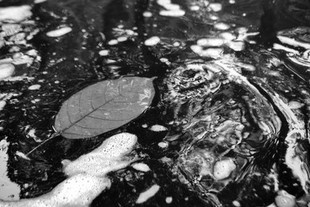
\includegraphics[width=\textwidth]{src.jpg}
        \caption{Figura original}
        \label{fig:src}
    \end{subfigure}
    \qquad
    \begin{subfigure}[ht]{0.45\textwidth}
        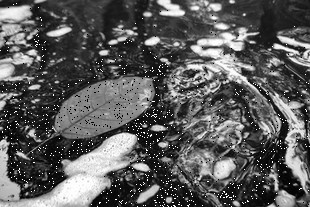
\includegraphics[width=\textwidth]{dst_sp.jpg}
        \caption{Com ruído \textit{salt and pepper}}
        \label{fig:salt_and_pepper}
    \end{subfigure}
    \caption{Imagem original e com filtro \textit{salt and pepper}}
\end{figure}

\subsubsection{Unipolar}
Se $P_a \cdot P_b = 0$ temos um ruído unipolar ja que apenas uma das faixas será modificada. Ou seja, apenas \pixels brancos ou pretos irão aparecer devido a neste tipo de ruído.

\subsection{Erlang}
A função de ditribuição de probabilidade Erlang foi originalmente desenvolvida para modelar trafego de ligações telefonicas.

\begin{equation}
p(z) = \left\{
    \begin{array}{l}
        \frac{a^{b}\cdot z^{b-1}}{(b - 1)!} \cdot e^{-a z} \text{ se } z \ge 0 \\
        0 \text{ se } z < 0
    \end{array}\right.
    \end{equation}

Onde $b$ é a forma e $a$ é a taxa de crescimento.

\subsubsection{Exponencial}
Se $b = 1$ temos um ruido exponencial

\begin{equation}
p(z) = \left\{
    \begin{array}{l}
        a \cdot e^{-a z} \text{ se } z \ge 0 \\
        0 \text{ se } z < 0
    \end{array}\right.
\end{equation}

\subsection{Rayleigh}
Como a função de distribuição de probabilidade de Rayleigh possui uma assimetria entre os lados direito e esquerdo, ela pode ser utilizada para aproximar histogramas assimétricos.

\begin{equation}
p(z) = \left\{
    \begin{array}{l}
        \frac{1}{b} \cdot (z - a) \cdot e^{\frac{-(z-a)^2}{b}} \text{ se } z \ge 0 \\
        0 \text{ se } z < 0
    \end{array}\right.
\end{equation}

\subsection{Uniforme}
A função distribuição de probabilidade uniforme eleva os níveis de cinza na faixa de $a$ até $b$

\begin{equation}
p(z) = \left\{
    \begin{array}{l}
        \frac{1}{b - a} \text{ se } a \le z \le b \\
        0 \text{ se } z < 0
    \end{array}\right.
\end{equation}

\subsection{Branco}
Quando o ruído em um \pixel $i$ é estatisticamente independente do ruído causado em um \pixel $j$, para quaisquer $i,j$, chamamos este ruído de branco. Matematicamente, ele é definido como um um conjunto de ruídos estatisticamente independentes com média zero e variância finita. Assim, sua covariância é zero. Em termos práticos, isto implica que qualquer \pixel da imagem pode receber um ruído de qualquer intensidade, independentemente do ruído recebido (ou não) pelos outros \pixels.

\subsection{Gaussiano}
Carioca

\section{Filtros espaciais de suavização}
Filtros de suavização são utilizados para enevoamento (\textit{blur}) e remoção de ruído. Estes filtros podem ser lineares ou não lineares. Dentre os lineares, destacam-se o filtro da média e o filtro gaussiano. Dentre os não-lineares, destaca-se o filtro da mediana.

\subsection{Filtro da média}
O filtro da média consiste em definir uma vizinhança e atribuir ao \pixel central a intensidade média dos \pixels desta vizinhança. A média pode tanto ser aritmética, em que cada \pixel tem o mesmo peso, como ponderada. Por exemplo, consideremos uma vizinhança $3\times3$. Para a média aritmética, temos que a máscara vale:

\[ w(s,t) = \frac{1}{9} \cdot \left|
    \begin{array}{ccc}
        1 & 1 & 1 \\
        1 & 1 & 1 \\
        1 & 1 & 1 \\
\end{array}\right|\]

Uma implementação possível para a máscara da média ponderada, para a mesma vizinhança, é dada por:

\[ w(s,t) = \frac{1}{16} \cdot \left|
    \begin{array}{ccc}
        1 & 2 & 1 \\
        2 & 4 & 2 \\
        1 & 2 & 1 \\
\end{array}\right|\]

Aplicou-se o filtro da média aritmética à Figura \ref{fig:src}, produzindo as imagens exibidas na Figura \ref{fig:avg_filter3} e \ref{fig:avg_filter5}.

\begin{figure}[!ht]
    \centering
    \begin{subfigure}[ht]{0.45\textwidth}
        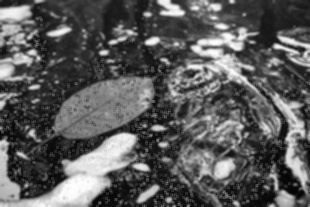
\includegraphics[width=\textwidth]{dst_sp_avg3.jpg}
        \caption{Janela $3 \times 3$}
        \label{fig:avg_filter3}
    \end{subfigure}
    \qquad
    \begin{subfigure}[ht]{0.45\textwidth}
        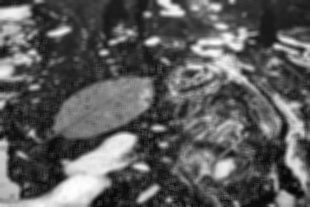
\includegraphics[width=\textwidth]{dst_sp_avg5.jpg}
        \caption{Janela $5 \times 5$}
        \label{fig:avg_filter5}
    \end{subfigure}
    \caption{Filtro da média (aritmética) aplicado à Figura \ref{fig:salt_and_pepper}.}
\end{figure}

\section{Filtros de domínio de frequência}
\subsection{Filtro Gaussiano}
Carioca

\section{Filtros estatísticos de ordem}
Filtros estatísticos de ordem são filtros não lineares que ordenam a intensidade dos \pixels do setor sendo considerando e estabelecem ao valor central desta área a intensidade do \pixel que esteja na $i$-ésima posição. Dentre estes, o mais comum é o filtro da mediana.

\subsection{Mediana}
Como o próprio nome sugere, o filtro da mediana substitui a intensidade de um \pixel pela intensidade da mediana de uma determinada vizinhança. Se por exemplo temos uma vizinhança $3\times3$, a mediana é o $5^o$ valor. Esta técnica é especialmente útil quando lidamos com ruídos do tipo \textit{salt and pepper}, já que este ruído é caracterizado justamente por possuir \pixels brancos ou pretos em locais inesperados e aleatórios. Assim, este filtro age forçando com que \pixels com intensidades discrepantes assumam valores mais próximos aos de seus vizinhos.

Aplicou-se o filtro da mediana com uma janela $3 \times 3$ à Figura \ref{fig:src}, produzindo as imagens exibidas na Figura \ref{fig:median_filter}. Verificamos que o filtro da mediana foi muito mais eficaz para eliminar os ruídos \textit{salt and pepper} do que o filtro da média, como já era esperado.

\begin{figure}[!ht]
    \centering
    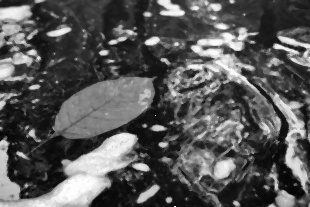
\includegraphics[width=0.45\textwidth]{dst_sp_median.jpg}
    \caption{Filtro da mediana aplicado à Figura \ref{fig:salt_and_pepper}}
    \label{fig:median_filter}
\end{figure}

\begin{thebibliography}{99}
    \bibitem{livro} GONZALEZ, Rafael C.; WOODS, Richard E.. \textbf{Digital Image Processing}. 3. ed. Upper Saddle River, NJ, EUA: Prentice-hall, 2006.
    \bibitem{whitenoise} \texttt{http://en.wikipedia.org/wiki/White\_noise}
\end{thebibliography}

\end{document}
